% !TEX encoding = UTF-8
% !TEX program = pdflatex
% !TEX spellcheck = it_IT

\documentclass[a4paper, 11pt]{article}

% sintassi
\usepackage[T1]{fontenc}
\usepackage[utf8]{inputenc}
\usepackage[english]{babel}
\DeclareUnicodeCharacter{00A0}{~}
\usepackage{fullpage}
%\usepackage[cochineal]{newtxmath}
%\usepackage{crimson,verbatim}
\usepackage[charter]{mathdesign}
\usepackage{textcomp}
\usepackage{color,soul,hyperref,mwe}

% matematica e chimica

\usepackage{siunitx,amsmath,bm,chemfig}
\newcommand{\ud}{\mathop{}\!\mathrm{d}}
\sisetup{detect-all,math-rm = \ensuremath}

\setatomsep{2em}

\newcommand\setpolymerdelim[2]{\def\delimleft{#1}\def\delimright{#2}} 
\def\makebraces[#1,#2]#3#4#5{% 
\edef\delimhalfdim{\the\dimexpr(#1+#2)/2}% 
\edef\delimvshift{\the\dimexpr(#1-#2)/2}% 
\chemmove{% 
\node[at=(#4),yshift=(\delimvshift)] {$\left\delimleft\vrule height\delimhalfdim depth\delimhalfdim 
width0pt\right.$};% 
\node[at=(#5),yshift=(\delimvshift)] 
{$\left.\vrule height\delimhalfdim depth\delimhalfdim 
width0pt\right\delimright_{\rlap{$\scriptstyle#3$}}$};}} 
\setpolymerdelim()

% tabelle e grafica
\usepackage{booktabs,graphicx,subfig,caption,pdfpages}
\captionsetup{font=small,
	format=hang,
	justification=centering,
	singlelinecheck=true,
	labelfont={sf,bf}	
}
\usepackage{float}
\usepackage[toc,page]{appendix}
\floatstyle{plaintop}
\restylefloat{table}
\usepackage{multirow}
\usepackage{fancyhdr}
\pagestyle{fancy}
\fancyhead[LE,RO]{\textsl{\rightmark}}
\fancyhead[LO,RE]{\nouppercase{\leftmark}}
\fancyfoot[C]{\thepage}
\usepackage[margin=1in,headsep=.3in]{geometry}
\usepackage[suftesi]{frontespizio}
\usepackage{xparse}
\setlength\parindent{0pt}

\newenvironment{chapterabstract}{%
  \par\nobreak\noindent
  \textbf{\textit{Abstract}\hrulefill}\nobreak
  %\small
  \noindent\ignorespaces
}{%
  \par\nobreak\normalsize
  \vskip-\ht\strutbox\noindent
  \textbf{\hrulefill}%
}
\makeatletter
\NewDocumentCommand\headerspdf{ O {pages=-} m }{% [options for include pdf]{filename.pdf}
  \includepdf[%
    #1,
    pagecommand={\thispagestyle{fancy}},
    scale=1,
    ]{#2}}
\NewDocumentCommand\secpdf{somO{1}m}{% [short title]{section title}[page specification]{filename.pdf} --- possibly starred
  \clearpage
  \thispagestyle{fancy}%
  \includepdf[%
    pages=#4,
    pagecommand={%
      \IfBooleanTF{#1}{%
        \section*{#3}}{%
        \IfNoValueTF{#2}{%
          \section{#3}}{%
          \section[#2]{#3}}}},
    scale=.65,
    ]%
    {#5}}
\makeatother

\begin{document}

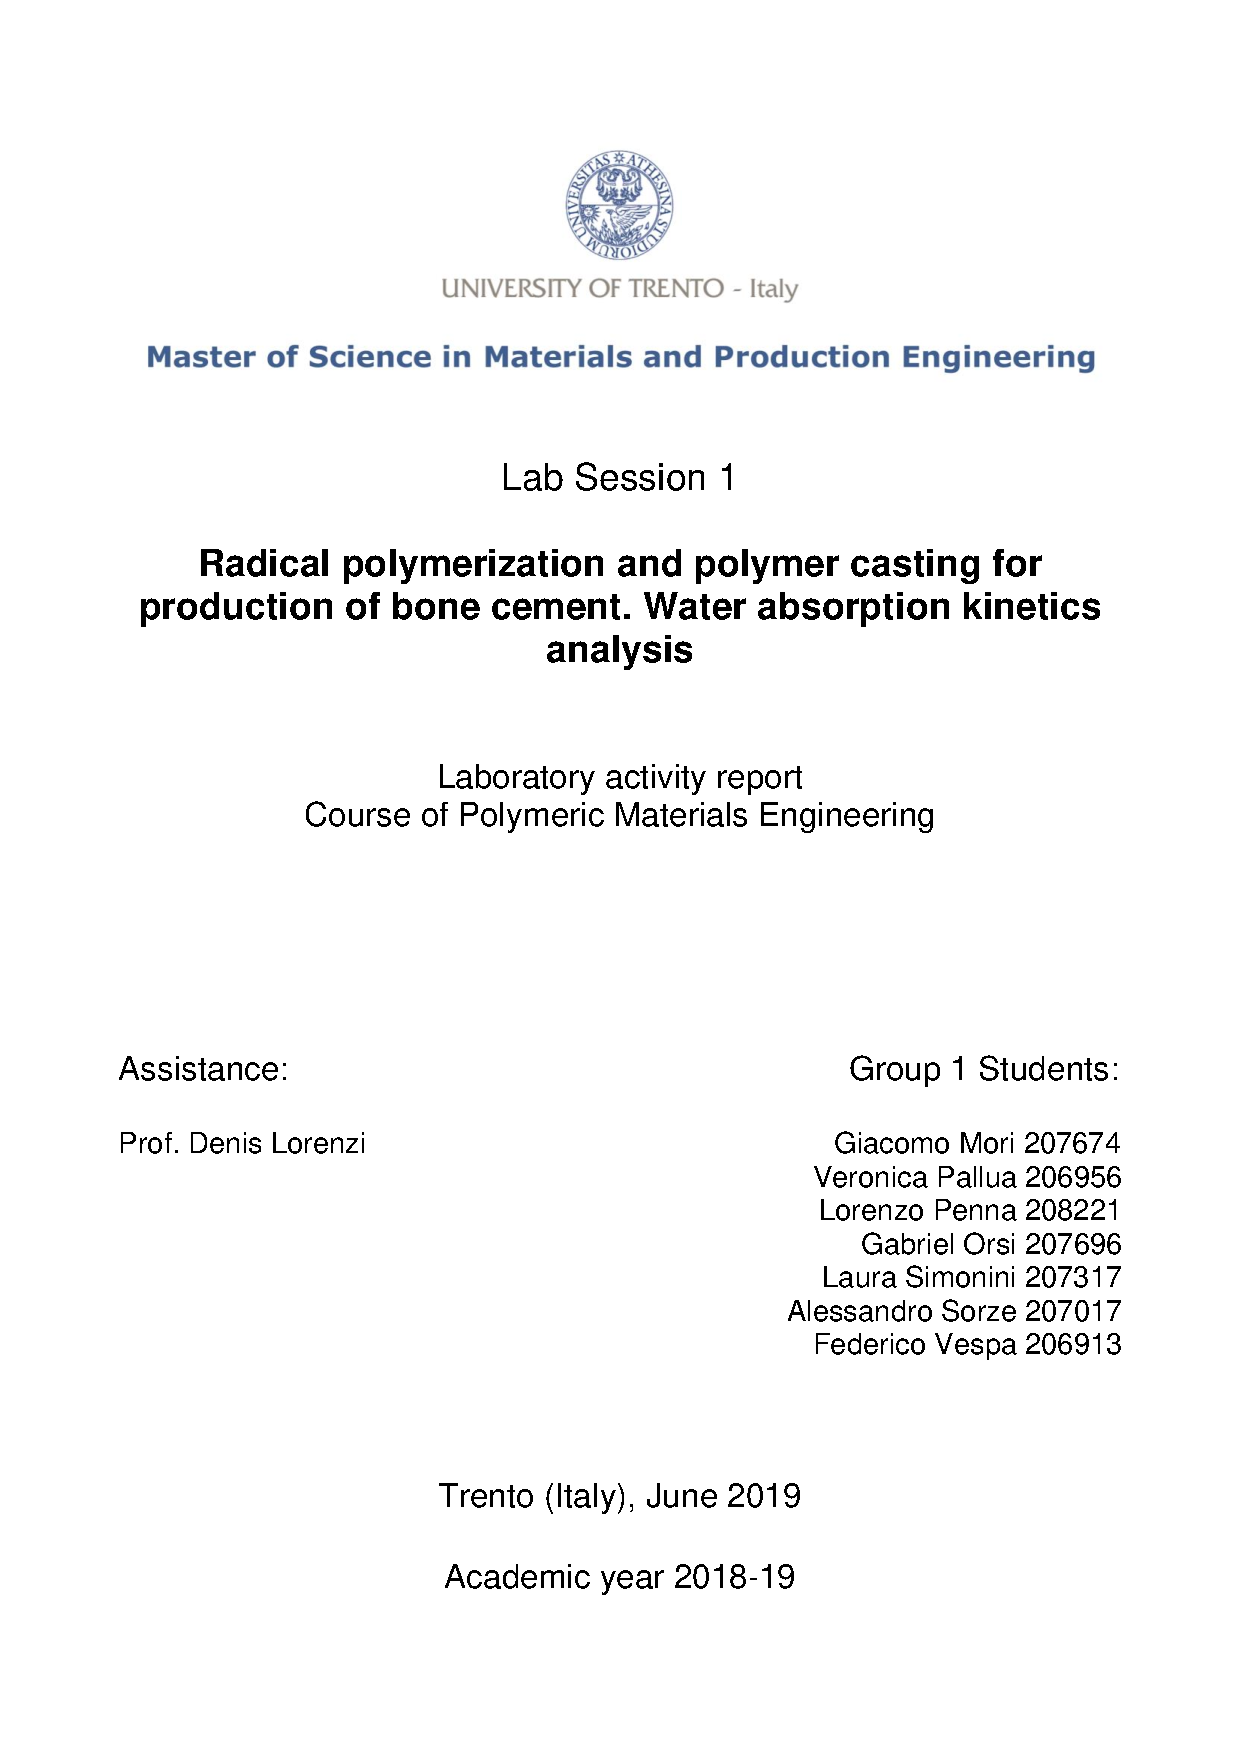
\includepdf[pages=-]{frontespizio1.pdf}

\begin{chapterabstract}

In this work a bone cement made of polymethyl methacrylate has been studied, paying attention to the heat released during polymerization and water absorption. The effect of the changed amount of monomer methyl methacrylate and the addition of a second monomer hydroxyethyl methacrylate have been studied. 

\end{chapterabstract} 

\section{Introduction}

The laboratory activity is concerned with radical polymerization of methyl methacrylate (MMA), used in biomedical applications for the production of bone cement. The analysis is aimed to evaluate heat of polymerization, the mass loss after heat treatment, the molecular weight of the polymerized samples and the water absorption in time. The composition of the bone cement has been modified by adding other monomer MMA and by adding a second monomer hydroxyethyl methacrylate (HEMA), to study the effects on previously cited experimental activities. 

\subsection {Materials}

In the powder the following components are present:
\begin{itemize}
\item Polymethyl methacrylate (MMA): acts as prepolymer which aim is to limit the increase of temperature produced by polymerization process. Moreover it increase the viscosity of the solution which allow an easier manipulation and descrease the degree of toxicity in the work environment. Another advantage of prepolymer is control the volumetric shrinkage during solidification.
\begin{figure}[h]
	\centering
	{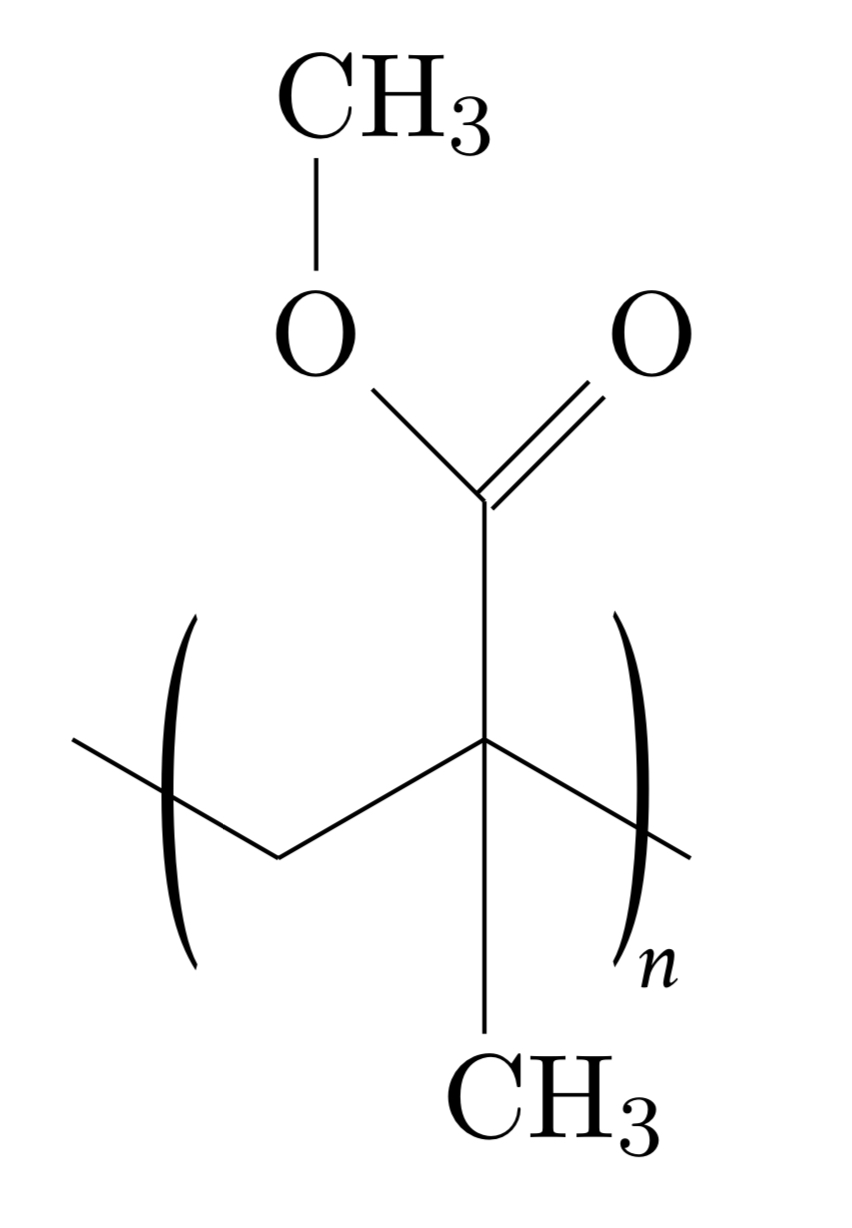
\includegraphics[scale=0.15]{pmma_chem}}
	\captionsetup{justification=centering}
	\label{fig:PE}
\end{figure}
\item Barium sulfate: is a radio opacifier because it allows the X-ray analysis.
\item Benzoyl peroxide (BPO): is the initiator infact it presents a bond between two atoms of oxygen that can be easily broken, producing two radicals.
\begin{figure}[h]
\centering
\chemfig{*6(-=-(-(=[2]O)-[::-60]O-[::60]O-[::-60](=[6]O)-(*6(-=-=-=)))=-=)} 
\end{figure}
\end{itemize}

\newpage

The liquid is composed by:
\begin{itemize}
\item Methyl methacrylate (MW = 104 g/mol): is the monomer involved in polymerization process. 
\begin{figure}[h!]
\centering
\chemfig{=[-0.6]([6]-)-[0.6](=[-6]O)-[-0.6]O-[0.6]} 
\end{figure}
\item N-N dimethyl-p-toluidine: acts as activator by breaking the BPO bond.
\item Hydroquinone: is a stabilizer to avoid the premature reaction of monomers.
\end{itemize}
Hydroxyethyl methacrylate (HEMA, MW = 130 g/mol): monomer able to absorb water due the presence of empty volumes in its structure. 
\begin{figure}[h]
\centering
\chemfig{=[-0.6]([6]-)-[0.6](=[-6]O)-[-0.6]O-[0.6]-[-0.6]-[0.6]OH} 
\end{figure}

\subsection{Radical addition polymerization}

In the experiment polymerization mechanism is radical addition. The activator for this reaction is N-N dimethyl-p-toluidine. The splitting of benzoyl peroxide, initiator of the reaction, provides two radicals and this leads to a subsequent addition of the monomers of methyl methacrylate. There are two different types of termination of the polymerization: combination and disproportional termination. In the first case two growing chains bind together, ending the polymerization, while in the second, through a reorganization of electrons, single polymeric chains end without any joint, producing multiple chains and less molecular weight.

\section{Materials and methods}

\subsection{Materials}

A medical kit Cemex Isoplastic High Viscosity for bone implants (bone cement) has been provided by Tecres Spa, Villafranca (IT). It is composed by two parts, a powder and a liquid, whose mixing produces the polymerization of reactants contained. In Table \ref{tab:kit} the nominal composition of the kit is reported. 
\begin{table}[htp]
\centering
$
\begin{array}{lc}
\toprule
\textbf{Component} & \textbf{Amount}\,(\%) \\
\midrule
\text{$40\si{g}$ of sterile powder containing:} & \\ 
\text{Polymethyl methacrylate} & 84.30  \\
\text{Barium sulphate} & 13.00  \\
\text{Benzoyl peroxide} & 2.70  \\
\midrule 
\text{$13.3\si{g}$ of sterile liquid containing:} & \\ 
\text{Methyl methacrylate} & 99.10  \\
\text{N-N dimethyl-p-toluidine} & 0.90  \\
\text{Hydroquinone} & 75\,\text{ppm}  \\
\bottomrule
\end{array}
$
\caption{Data-sheet of Cemex Isoplastic High Viscosity.}
\label{tab:kit}
\end{table}\\
Additional methyl methacrylate monomer has been provided by University of Trento, together with hydroxyethyl methacrylate monomer. 

\newpage

\subsection{Sample preparation}

Parts contained in the medical kit has been weighted with instrument Mettler PM460 (sens. $\pm 0.001\,\text{g}$). Both full and empty containers of the powder and the liquid has been weighted, in order to have a feedback of possible losses of material. Disposable bowls and rods in polyethylene (PE), provided along with the kit, have been weighted as well, and used for the preparation of samples. Reagents have been poured in the bowl, first putting the powder and then the liquid, and stirred vigorously with the rod, till the viscosity of the system was enough to allow for manipulation and formation of samples: a spherical one and a defined number of sticks, that have been pressed in a polytetrafluoroethylene (PTFE) mold. Prior to the beginning of the polymerization, the spheroid has been weighted for subsequent heat of polymerization measurments. A thermometer has been inserted inside the spheroid interposing an aluminum foil, to prevent the direct contact with the reacting polymer and avoiding sticking effects. The system including the thermometer has been put quickly in a chamber full of expanded polystyrene (EPS) and an aluminum foil has been wrapped around of it, to minimize heat losses and to get a more precise measurement of temperature variation. Measurements of temperature has been taken as polymerization process occured, until the achievement of maximum temperature. Moreover, a few further temperature measurements have been taken after the pick to highlight the shape of the temperature-time curve. Four sticks, once polymerized, have been cured at $90^\circ$C for 10 minutes and subsequently weighted in order to report for mass losses due to polymerization and evaporation of liquid monomer. All stick and spheroid samples have been soaked in water to study the water absorption of the material. 
In Table \ref{tab:code} coding for samples is reported. 
\begin{table}[htp]
\centering
$
\begin{tabular}{ll}
\toprule
\textbf{Code} & \textbf{Description} \\
\midrule
P1HT & stick, first polymerization, heat treatment\\ 
P1 & stick, first polymerization, without heat treatment\\
P2HT & stick, second polymerization, heat treatment\\
P2 & stick, second polymerization, without heat treatment\\
S1 & spheroid, first polymerization, without heat treatment\\
S2 & spheroid, second polymerization, without heat treatment\\
S3 & spheroid, third polymerization, without heat treatment\\
\bottomrule
\end{tabular}
$
\caption{Sample coding.}
\label{tab:code}
\end{table}\\

In Table \ref{tab:compos} the compositions of spheroids used for the calculations are reported. For each value, the percentage respect to spheroid mass is reported.
\begin{table}[htp]
\centering
$
\begin{array}{lccc}
\toprule
& \textbf{P1} & \textbf{P2} & \textbf{P3}  \\
\midrule
\mathbf{m_{PMMA}}\,(\text{g}) & 20.62\ (62.7\%) & 21.65\ (55.2\%) & 8.69\ (62.6\%) \\
\mathbf{m_{BaSO_4}}\,(\text{g}) & 3.18\ (9.7\%) & 3.34\ (8.5\%) & 1.34\ (9.6\%) \\
\mathbf{m_{BPO}}\,(\text{g}) & 0.66\ (2\%) & 0.70\ (1.8\%) & 0.28\ (2\%) \\
\mathbf{m_{MMA}}\,(\text{g}) & 8.35\ (25.4\%) & 10.72\ (27.3\%) & 3.55\ (25.5\%) \\
\mathbf{m_{HEMA}}\,(\text{g}) & - & 2.74\ (7\%) & - \\
\mathbf{m_{activator}}\,(\text{g}) & 0.075\ (0.2\%) & 0.08\ (0.2\%) & 0.03\ (0.2\%) \\
\mathbf{m_{stabilizer}}\,(\text{ppm}) & 46.88 & 49.3 & 19.76 \\
\midrule
\mathbf{m_{spheroid}}\,(\text{g}) & 32.89 (100\%) & 39.23
\ (100\%) & 13.90\ (100\%) \\
\bottomrule
\end{array}
$
\caption{Compositions of spheroids for each polymerization.}
\label{tab:compos}
\end{table}\\


\subsubsection{Estimation of sticks number}

The number of obtainable sticks has been calculated considering shape, dimensions 
of molds, density ($1.5\,\text{g/cm}^3$) and weigth of the whole kit.
The ratio between the total volume of mixture and the volume of a mold gives the theoretical number of possible sticks that is equal to 8 with width of $10.15\,\text{mm}$, lenght $130.04\,\text{mm}$ and thickness $3.30\,\text{mm}$.
However part of mixture has been used for the preparation of spheroid and thus the number of sticks produced is less.

\section{Experimental activity}

Three polymerizations have been carried out: 
\begin{enumerate}
\item using the medical kit as provided;
\item using the medical kit and adding about $3 \text{ml}$ of MMA and $4 \text{ml}$ of HEMA;
\item using the medical kit as provided, like as in case 1, but producing more sticks and thus a smaller spheroid.
\end{enumerate}

\subsection{Heat of polymerization measurements}

Heat of polymerization $\Delta H \,(\text{J})$ has been measured accordingly to the Equation \ref{eq:heat}:
\begin{equation}
\Delta H = m \,c_p \Delta T
\label{eq:heat} 
\end{equation}
Where $c_p$ ($\frac{\text{J}}{\text{g}^\circ\text{C}}$) is the specific thermal capacity of polymethyl methacrylate, $m$ is the mass of the spheroid and $\Delta T\,(^\circ\text{C})$ is the temperature variation measured during polymerization, taken as the difference between maximum reached and room one. Specific heat of polymerization $\Delta H_{sp}\,(\text{J}/\text{g} \,\, \text{and} \,\, \text{kJ}/\text{mol})$ has been calculated accordingly to the Equation \ref{eq:spheat}:
\begin{equation}
\Delta H_{sp} = \frac{\Delta H}{m_{mon}}
\label{eq:spheat} 
\end{equation}
Where $m_{mon}$ is the mass of the monomers. \\
In the case of copolymerization of MMA and HEMA, the specific heat has been calculated with Equation \ref{eq:copoly}:
\begin{equation}
\Delta H_{sp} = \Delta H_{sp}^\text{MMA} + \Delta H_{sp}^\text{HEMA}
\label{eq:copoly} 
\end{equation}
Where $\Delta H_{sp}^\text{MMA}$ is the specific heat of polymerization of MMA and $\Delta H_{sp}^\text{HEMA}$ is the specific heat of polymerization of HEMA. To calculate the specific enthalpy of reagents in kJ/mol, the weighted average of the molecular weights of the two monomers has been used.

\subsection{Estimation of polymer molecular weight}

Polymer molecular weight MW can be expressed by Equation \ref{eq:mw}:
\begin{equation}
\text{MW} = \text{DP}\cdot m_{mon}
\label{eq:mw} 
\end{equation}
Where DP is the degree of polymerization and $m_{mon}\,(\text{g}/\text{mol})$ is the molar mass of the monomer. The degree of polymerization has been found relating the amount of monomer $n_{mon}\,(\text{mol})$ with the amount of radicals of benzoyl peroxide $n_{rad}\,(\text{mol})$, as in Equation \ref{eq:dp}.
\begin{equation}
\text{DP} = \frac{n_{mon}}{n_{rad}}
\label{eq:dp} 
\end{equation}


The amount of radicals is equal to double the amount of BPO, due to the peroxide dissociation. Equation \ref{eq:dp} is suitable for the calculation of the degree of polymerization in case of disproportional termination. In case of combination, DP is the double. In a third case, the average of these two DP values has been also evaluated since it represents a more realistic case (MW 50\% - 50\%).\\
In the second polymerization, it has been considered also the contribution of HEMA according to Equations \ref{eq:dp2} and \ref{eq:mw2}.
\begin{equation}
\text{DP} = \frac{n_\textup{MMA} + n_\textup{HEMA}}{n_{rad}}
\label{eq:dp2} 
\end{equation}
Where $n_\textup{MMA}$ is the number of moles of MMA in the spheroid, $n_\textup{HEMA}$ the number of moles of HEMA in spheroid.
\begin{equation}
\text{MW} = \text{DP}\cdot m^*_{mon}
\label{eq:mw2} 
\end{equation}
In this case $m^*_{mon}$ is the weighted mean of molecular weights of MMA ($100\,\text{g/mol}$) and HEMA ($130\,\text{g/mol}$). \par 
In both cases, for Flory principle, different chains have been supposed to have same propagation speed during polymerization. 

\subsection{Effect of heat treatment after polymerization}

Heat treatment has been done by curing samples at $90^\circ$C for 10 minutes, using the instrument Mettler Thermobalance LP16. The percent mass loss has been calculated with Equation \ref{eq:htreat}.
\begin{equation}
\%\text{wt loss} = \frac{m_{cured}-m_0}{m_0}\cdot 100
\label{eq:htreat} 
\end{equation}
Where $m_{cured}$ is the mass after the heat treatment and $m_0$ is the initial mass just after polymerization. 

\subsection{Water absorption measurements}

Water absorption has been calculated accordingly to Equation \ref{eq:wabs}.
\begin{equation}
\%\text{water abs} = \frac{m_{wet}-m_0}{m_0}\cdot 100
\label{eq:wabs} 
\end{equation}
Where $m_{wet}$ is the mass after soaking and careful removal of superficial film of water. Different measurements of $m_{wet}$ have been taken over the period of one month, allowing for the plot of the water absorption curve with time. Sampling was more frequent in the initial period, while measurements progressively became more sparse in the final one. 

\subsubsection{Drying of samples after water soaking}

Samples after water absorption of three months (90 days) have been subjected to a drying process in oven at 85°C for 96 hours. The samples have been weighted with instrument Mettler PM460 (sens. $\pm 0.001\,\text{g}$) and the weight loss percent reported. 

\newpage
\section{Results and discussion}

\subsection{Heat of polymerization measurements}

In Table \ref{tab:heat} heat of polymerization results are reported. 
\begin{table}[htp]
\centering
$
\begin{array}{ccccccc}
\toprule
\textbf{Sample} & \mathbf{\Delta T}\,(\text{K}) &  \mathbf{m}\,(\text{g}) & \mathbf{\Delta H}\,(\text{J}) & \mathbf{\Delta H_{sp}}\,(\text{J}/\text{g}) & \mathbf{\Delta H_{sp}^{MMA}}\,(\text{kJ}/\text{mol}) & \mathbf{\Delta H_{sp}^{HEMA}}\,(\text{kJ}/\text{mol}) \\
\midrule
\text{S1} & 78 & 32.9 & 3848 & 461 & 46.1 & -\\
\text{S2} & 81 & 39.2 & 4767 & 354 & 46.1 & - 8.93 \\
\text{S3} & 62 & 13.9 & 1292 & 364 & 36.4 & - \\
\bottomrule
\end{array}
$
\caption{Calculated heat of polymerization.}
\label{tab:heat}
\end{table}\\
Specific thermal capacity of PMMA has been fixed at $1.5 \,\frac{\text{J}}{\text{g}^\circ\text{C}}$.
The specific heat of MMA for the second polymerization has been taken equal to the first polymerization, in order to calculate the contribution in specific heat of the HEMA monomer. From Table \ref{tab:heat} it can be noticed how the heat of polymerization of the second case is way larger than the first, due to the added amount of MMA monomer. The specific heat of HEMA has been found to be negative and this is probably due to errors during measurements: the kinetic of second polymerization reaction was so fast that at the beginning it was not possible to avoid some heat losses. Between the first and third case, the heat of polymerization is comparable, although smaller. This can be partially explained by the higher surface/volume ratio of the smaller spheroid in the third experiment: heat exchange with environment is greater and, together with a possible poorer insulation of the chamber, a lower measured temperature variation is produced ($85^\circ$C of pick where in the first case it was $101^\circ$C). \\
In Figure \ref{fig:Tt} the charts reporting temperature ramp over time for three polymerizations are reported. 
\begin{figure}[htp]
\centering
{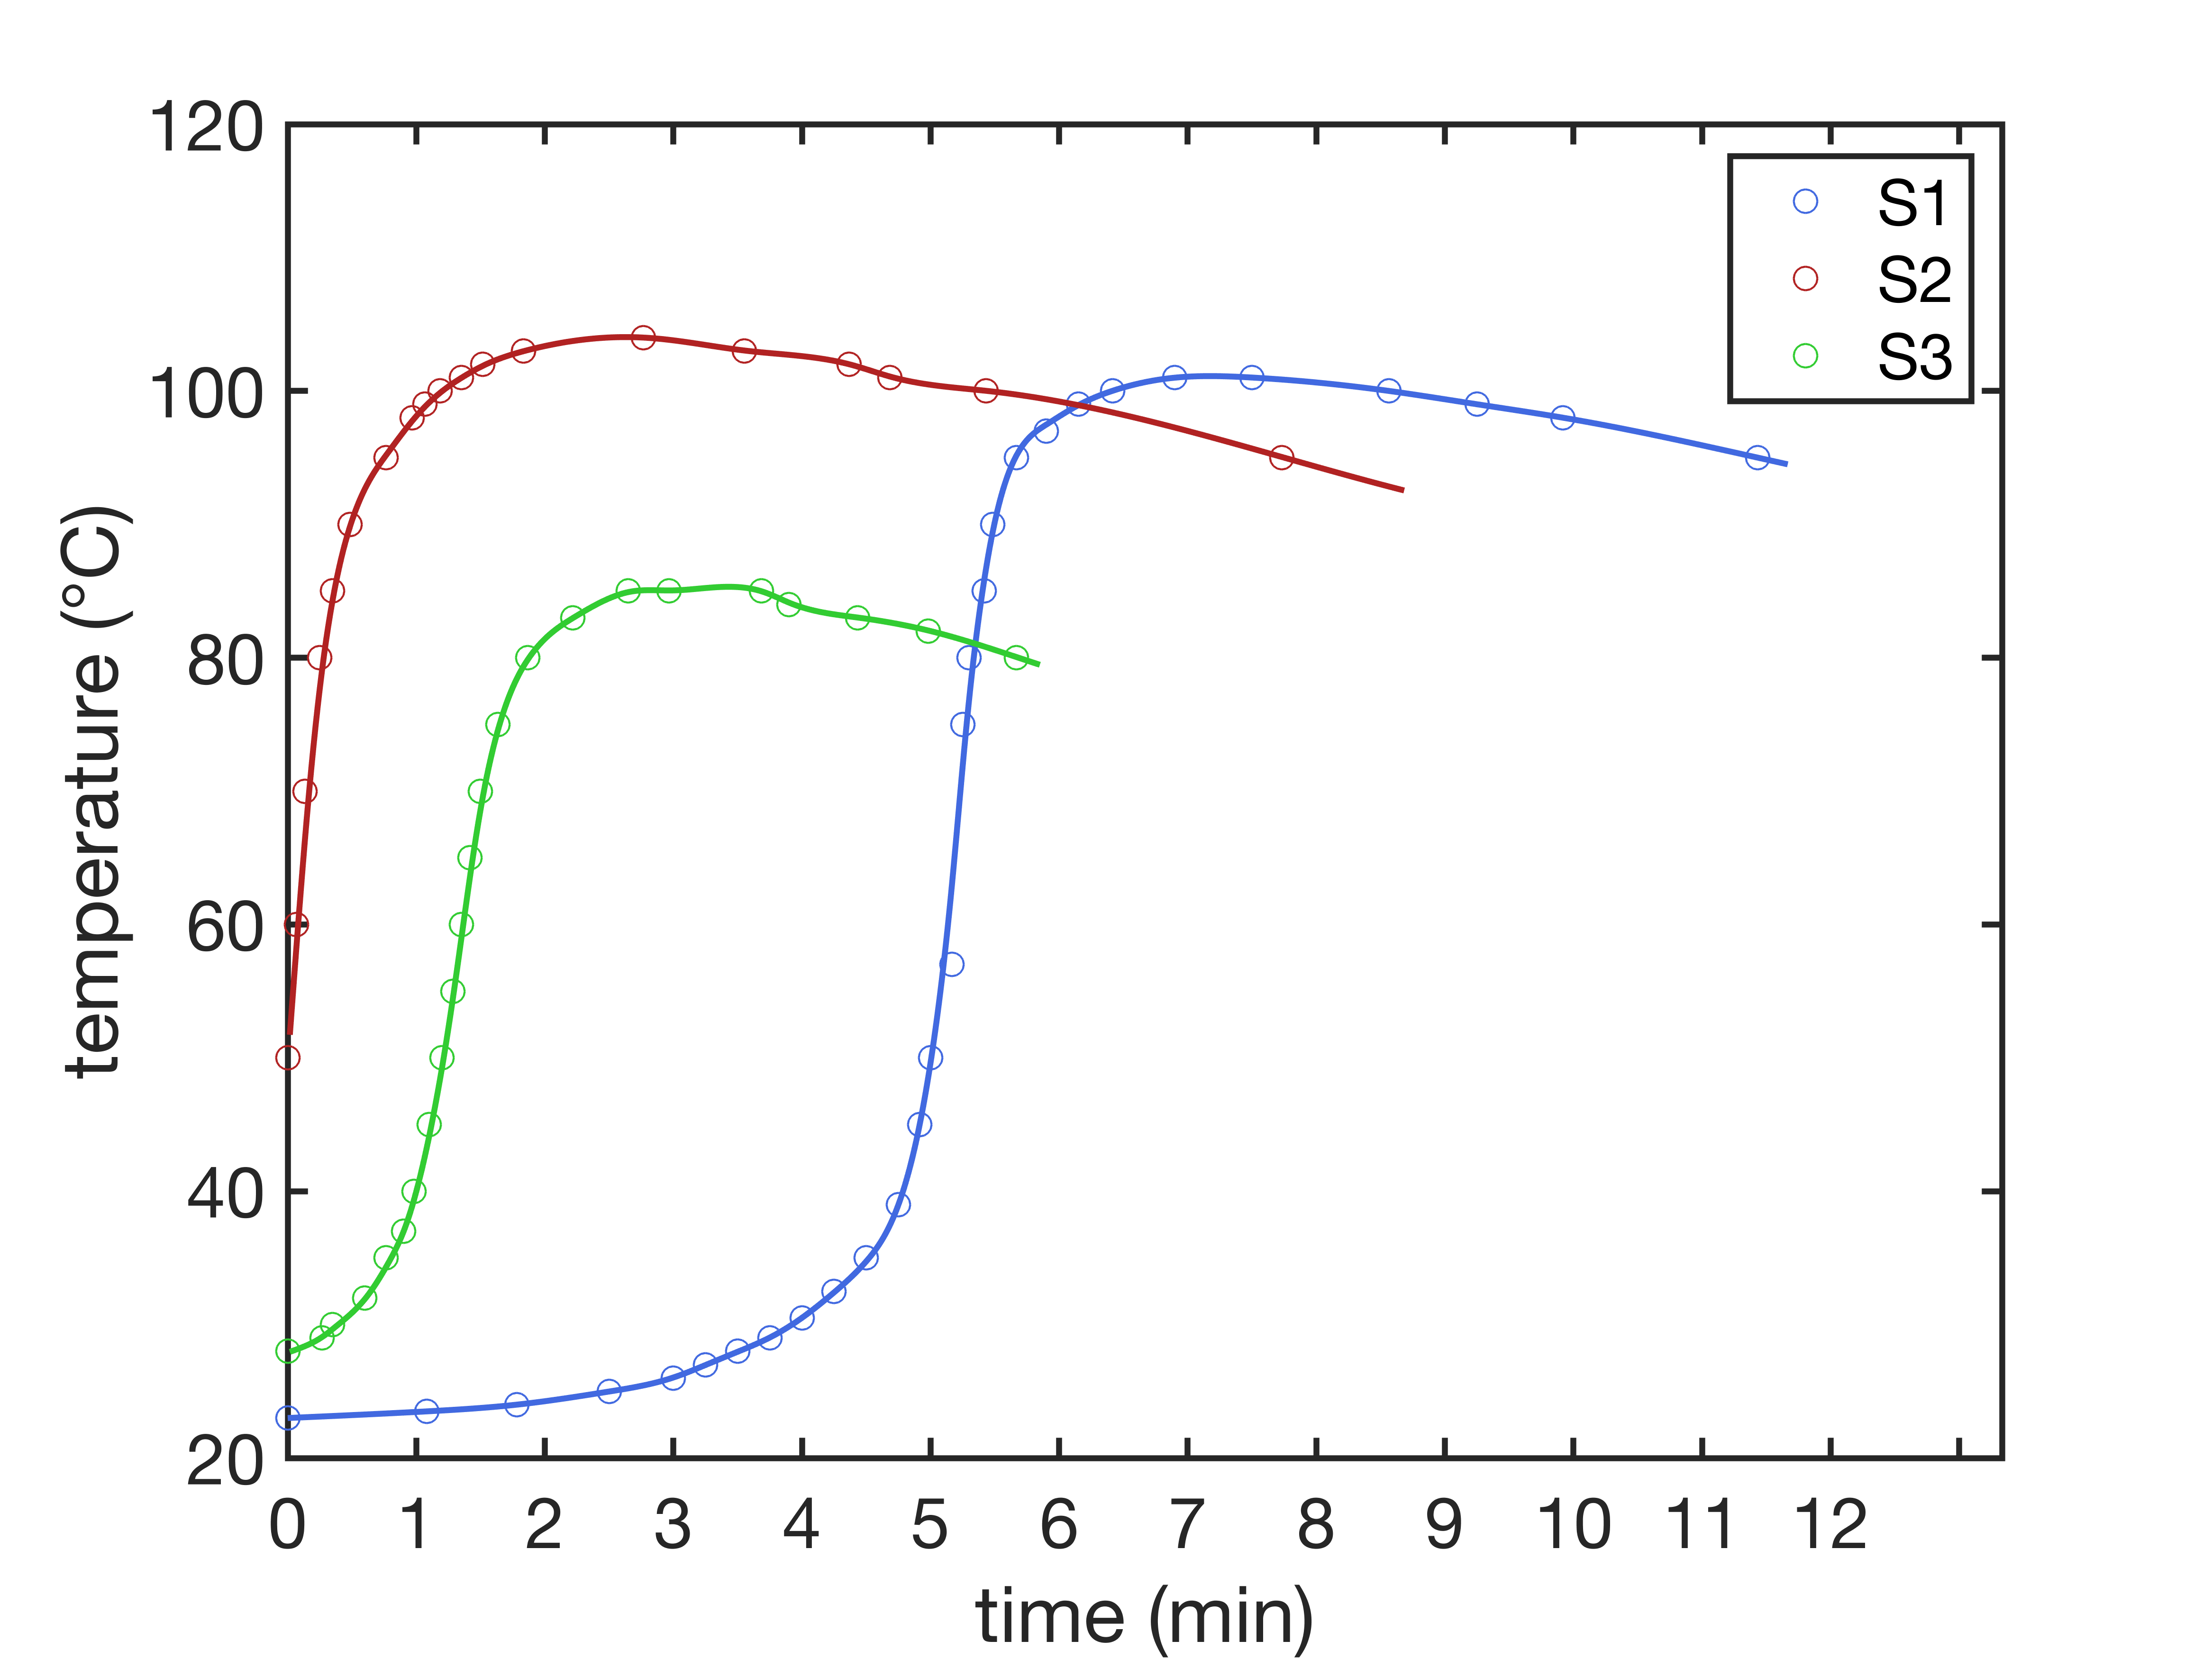
\includegraphics[scale=0.35]{heatrelease}}
\captionsetup{justification=centering}
\caption{Time-temperature charts for S1 S2 and S3 samples.}
\label{fig:Tt}
\end{figure}\\

\newpage

\subsection{Estimation of polymer molecular weight}

In the following Table \ref{tab:dp} the degree of polymerization for every reaction is reported, calculated according to Equation \ref{eq:dp}.
\begin{table}[htp]
\centering
$
\begin{array}{cccc}
\toprule
& \textbf{S1} & \textbf{S2} & \textbf{S3}  \\
\midrule
\textbf{DP} & 16 & 22 & 16 \\
\bottomrule
\end{array}
$
\caption{Degree of polymerization for the three spheroidal samples.}
\label{tab:dp}
\end{table}\\
It can be noticed that the degree of polymerization is higher for the second polymerization reaction due to the larger amount of the monomer MMA.

In Table \ref{tab:mw}, molecular weights for each type of termination are reported. They are referred to the three polymerizations and have been calculated according to Equation \ref{eq:mw}.

\begin{table}[htp]
\centering
$
\begin{array}{cccc}
\toprule
\textbf{Sample} & \textbf{MW}\,(\text{g/mol}) & \textbf{MW}\,(\text{g/mol}) & \textbf{MW}\,(\text{g/mol}) \\
& \text{disproportional 100\%} & \text{combination 100\%} & \text{50\% - 50\%} \\
\midrule
\text{S1} & 1558 & 3116 & 2337 \\
\text{S2} & 2364 & 4729 & 3547 \\
\text{S3} & 1546 & 3092 & 2319 \\
\bottomrule
\end{array}
$
\caption{Molecular weights for each type of termination.}
\label{tab:mw}
\end{table}

In the first and third case results are very similar beacuse the amount of MMA is the same. For the second polymerization, instead, the value of molecular weight is higher since a larger quantity of monomer is present.

\subsection{Effect of heat treatment after polymerization}

In Table \ref{tab:heattr} the results of the heat treatment on weight are reported.
\begin{table}[htp]
\centering
$
\begin{array}{cc}
\toprule
\textbf{Sample} & \textbf{$\%$mass loss}  \\
\midrule
\text{P1HT} & 0.13\pm0.01 \\
\text{P2HT} & 0.10\pm0.03 \\
\bottomrule
\end{array}
$
\caption{Heat treatment mass loss measurements.}
\label{tab:heattr}
\end{table}\\
From the Table it can be stated how the mass loss is around 0.1\% for both cases, indicating a non preferential evaporation of the HEMA containing samples. These mass losses are related to the evaporation of the non polymerized monomers, still in liquid state and with an evaporation point of $101^\circ$C, very close to the heat treatment temperature. The sligthly less weight loss of the P2HT are due to the much higher evaporation point of HEMA, around $213^\circ$C, with poor or no evaporation at all during the process. 
\newpage
\subsection{Water absorption measurements}

In Figure \ref{fig:wabs1} the charts reporting water absorption over time for first and second polymerizations are reported, considering stick samples and dividing samples which underwent the heat treatment from the others. 
\begin{figure}[htp]
\centering
\subfloat[][]
{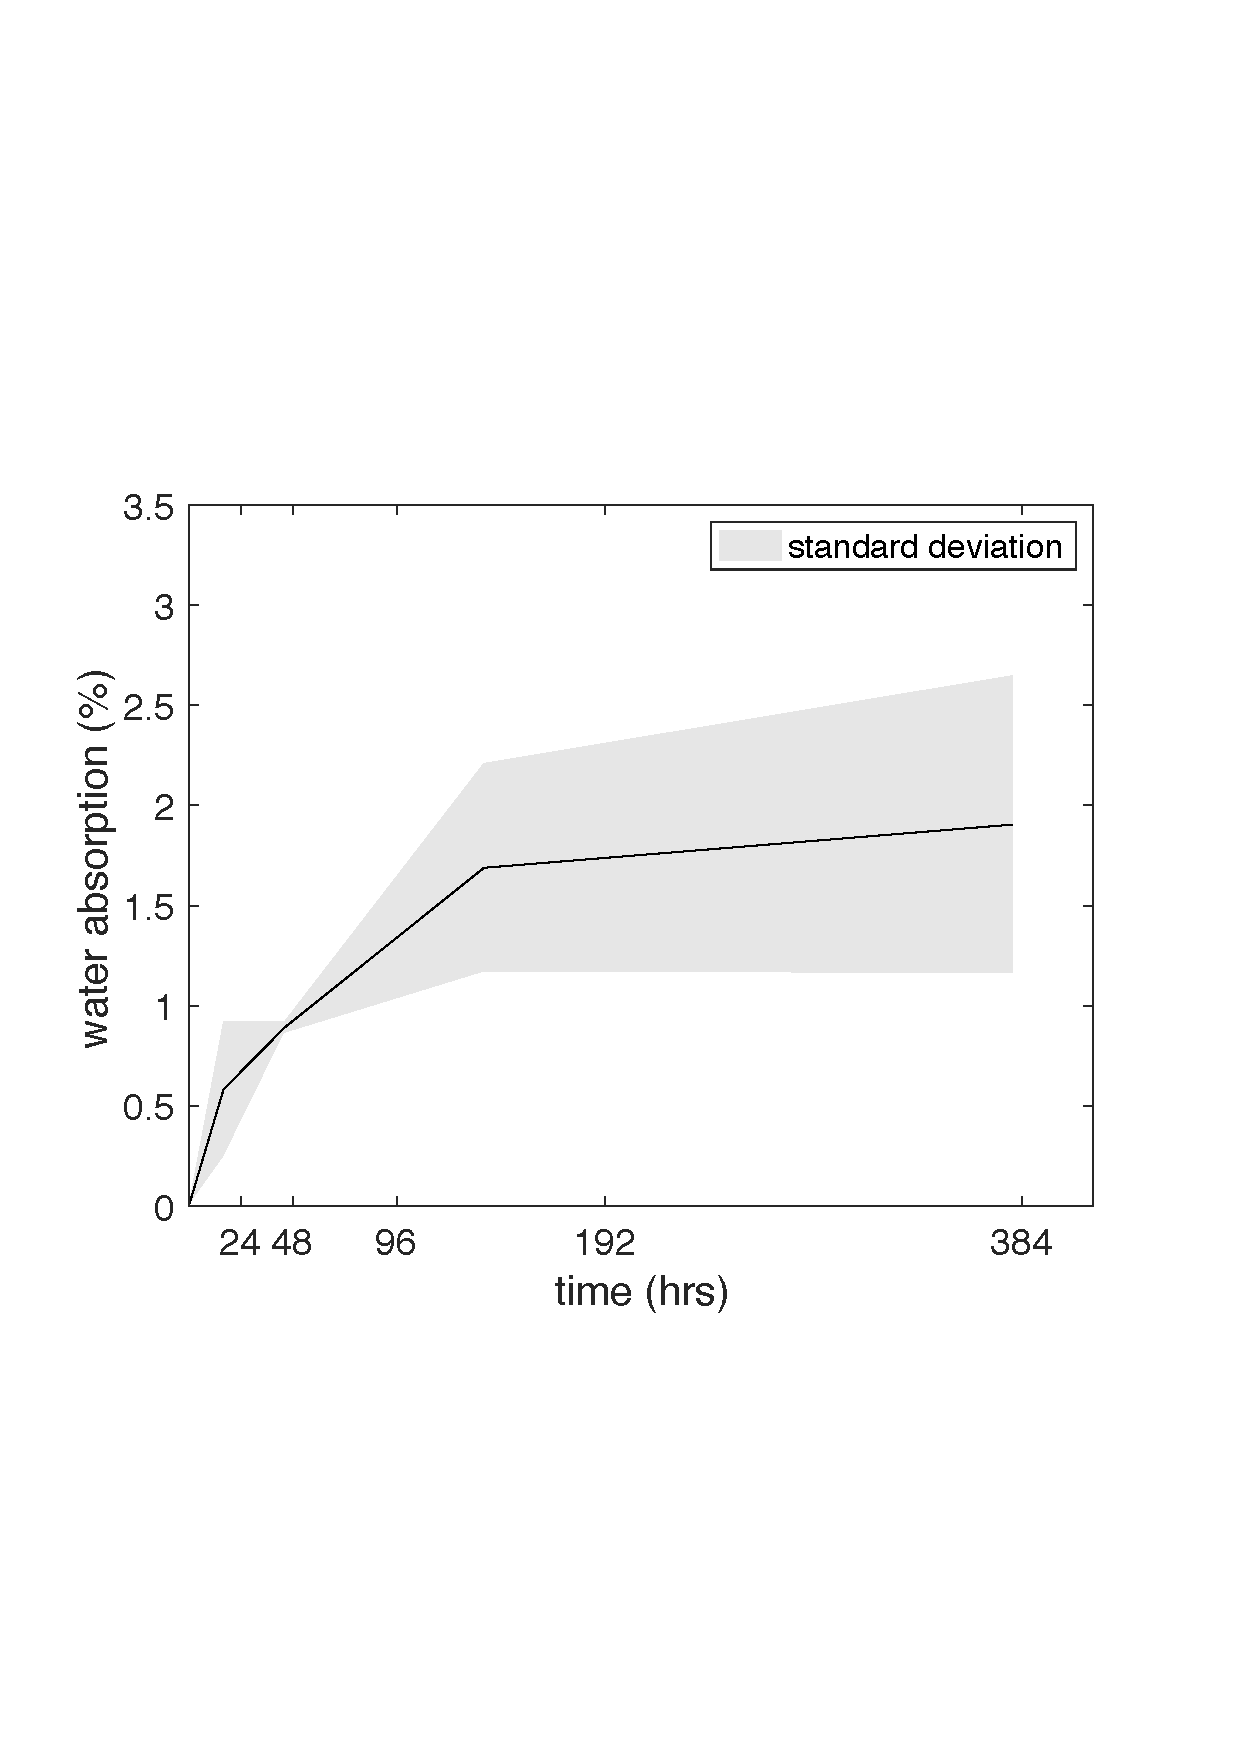
\includegraphics[scale=0.35]{wabs1}} \quad 
\subfloat[][]
{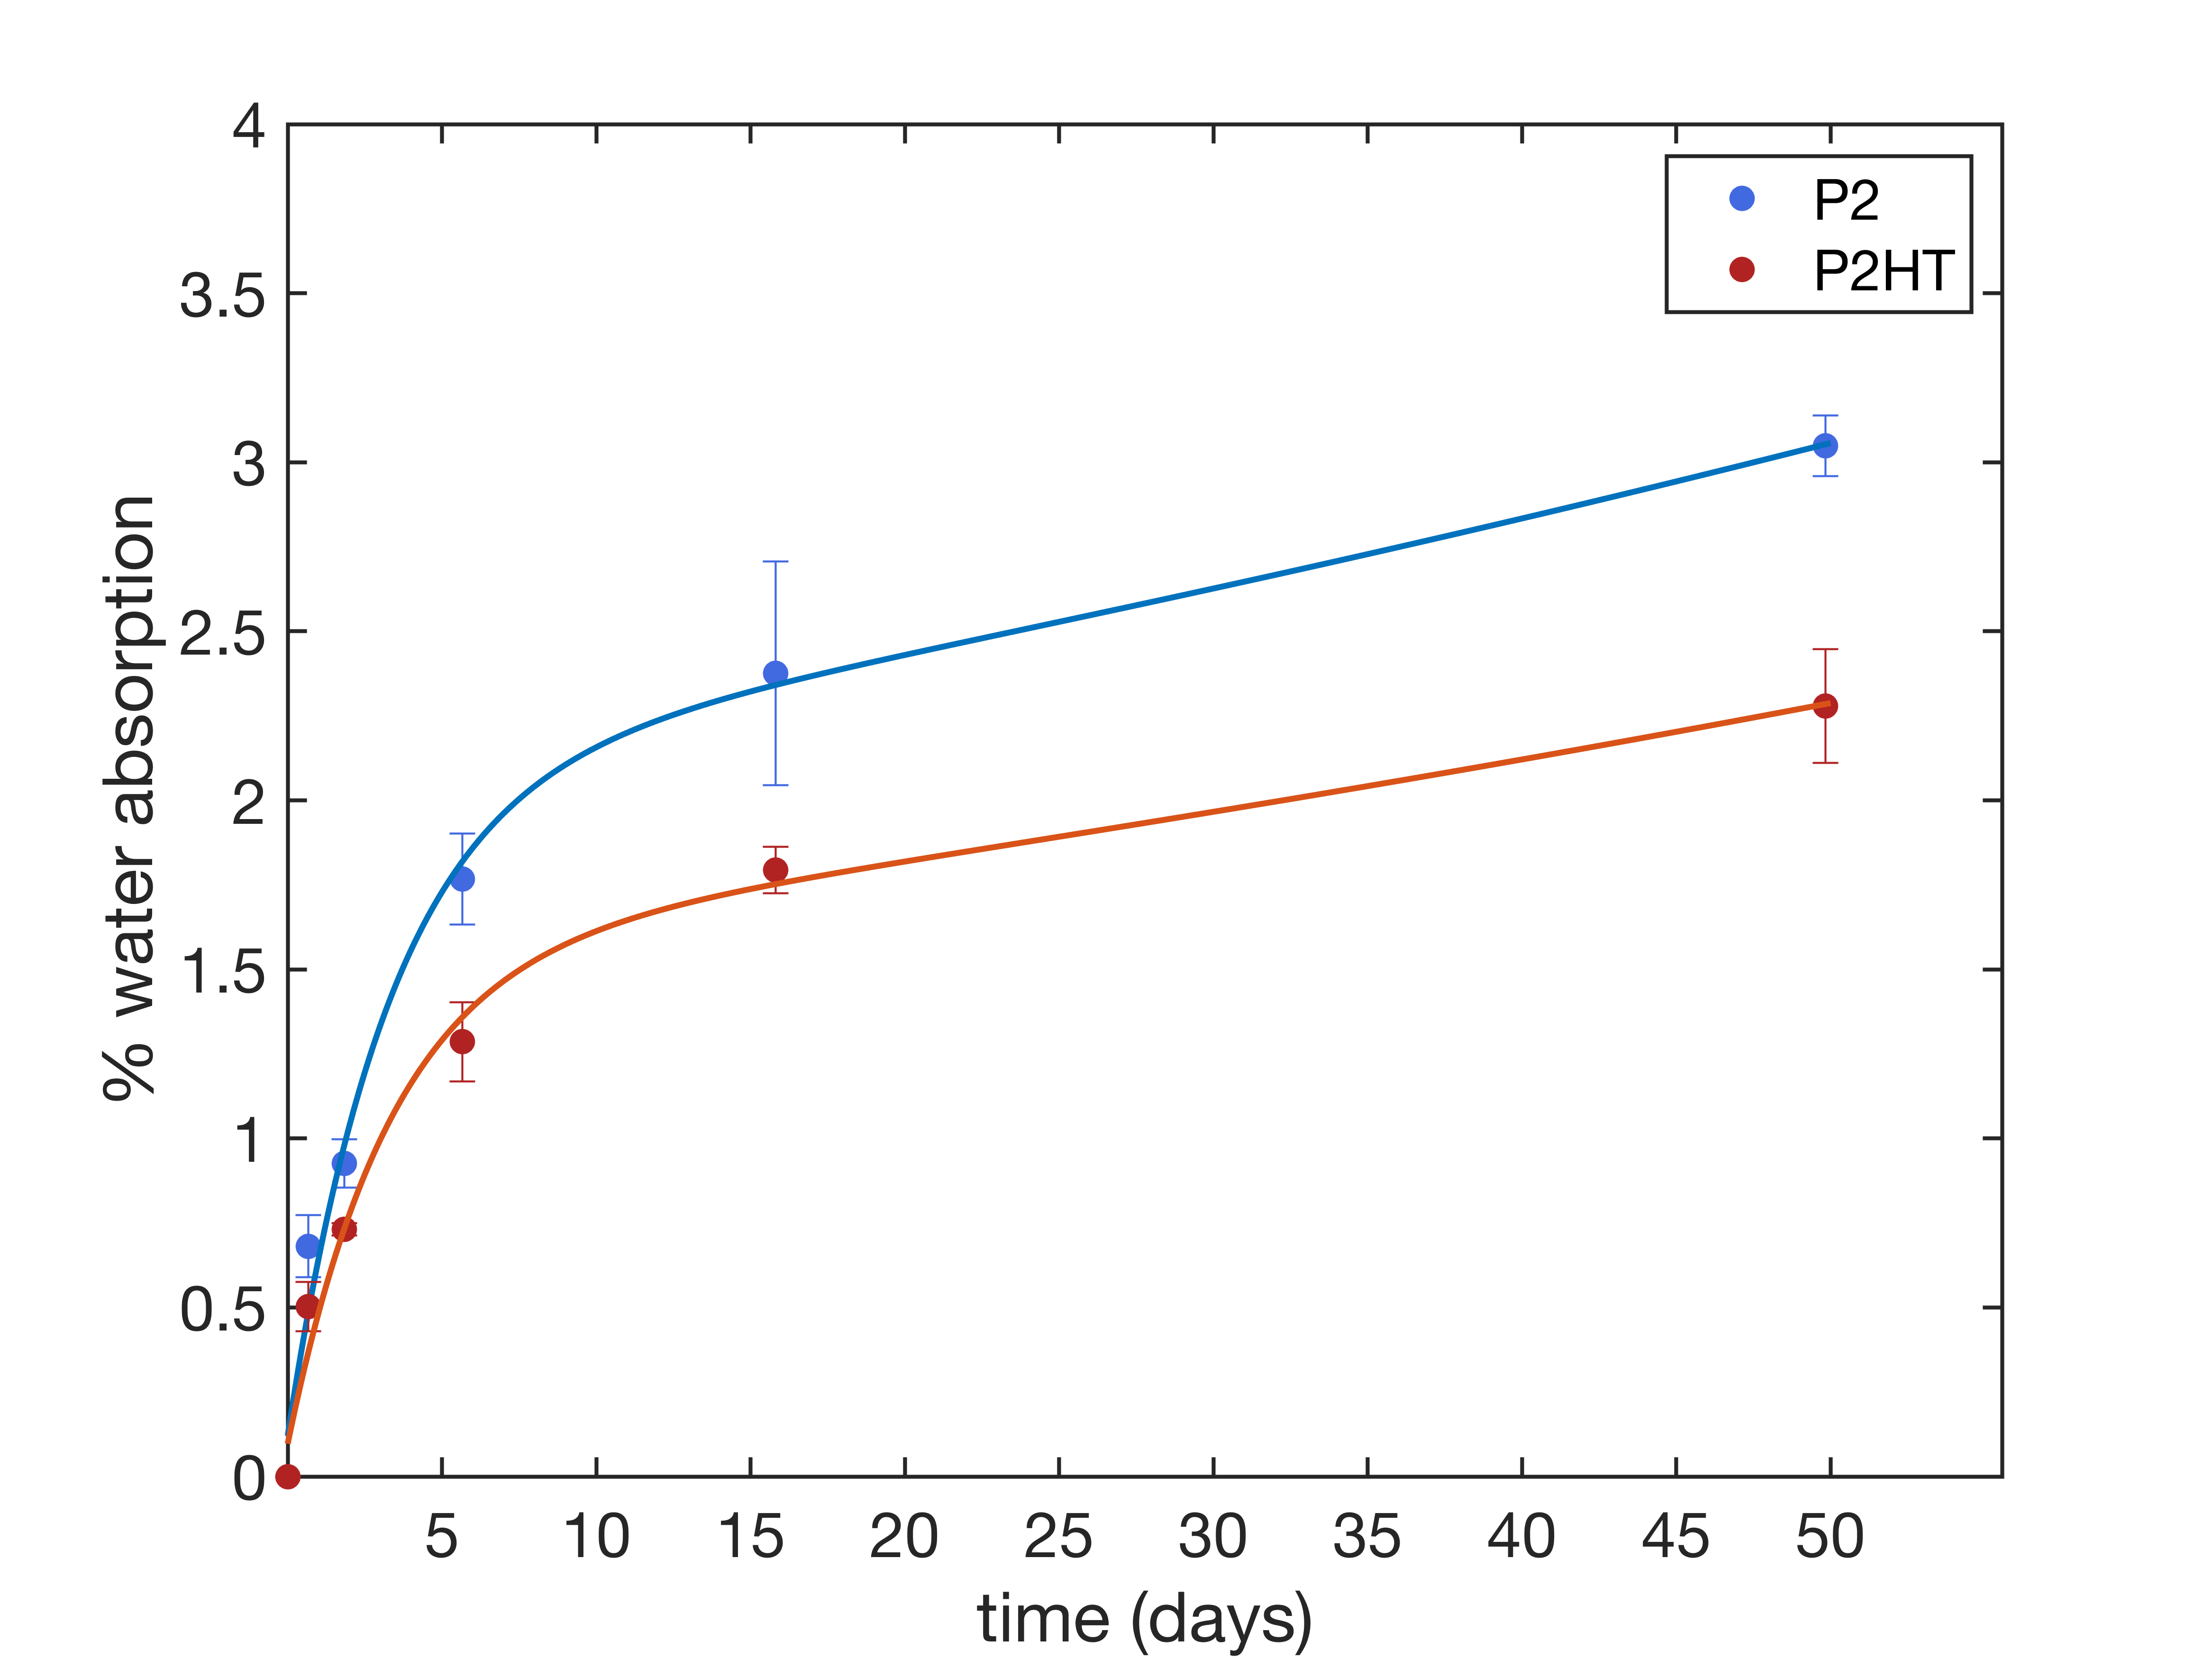
\includegraphics[scale=0.35]{wabs2}}
\captionsetup{justification=centering}
\caption{Water absorption curves for: (a) P1 and (b) P2.}
\label{fig:wabs1}
\end{figure}\\
From charts it can be stated how the presence of HEMA increases the water absorption, while the heat treatment has as opposite effect, reducing the amount of water absorbed by PMMA. These effects are justified by the presence of OH groups in the HEMA monomer, that are responsible of enhanced hydrophilicity of the final polymer. On the other side, the heat treatment seems to be related to a smaller hydrophilicity, probably due to the partial evaporation of non-polymerized monomer and for the higher degree of polymerization induced by an increase of temperature and thus the kinetics. \\
In Figure \ref{fig:wabs2} the charts reporting water absorption over time for the three polymerizations are reported, considering spheroidal samples. 
\begin{figure}[htp]
\centering
{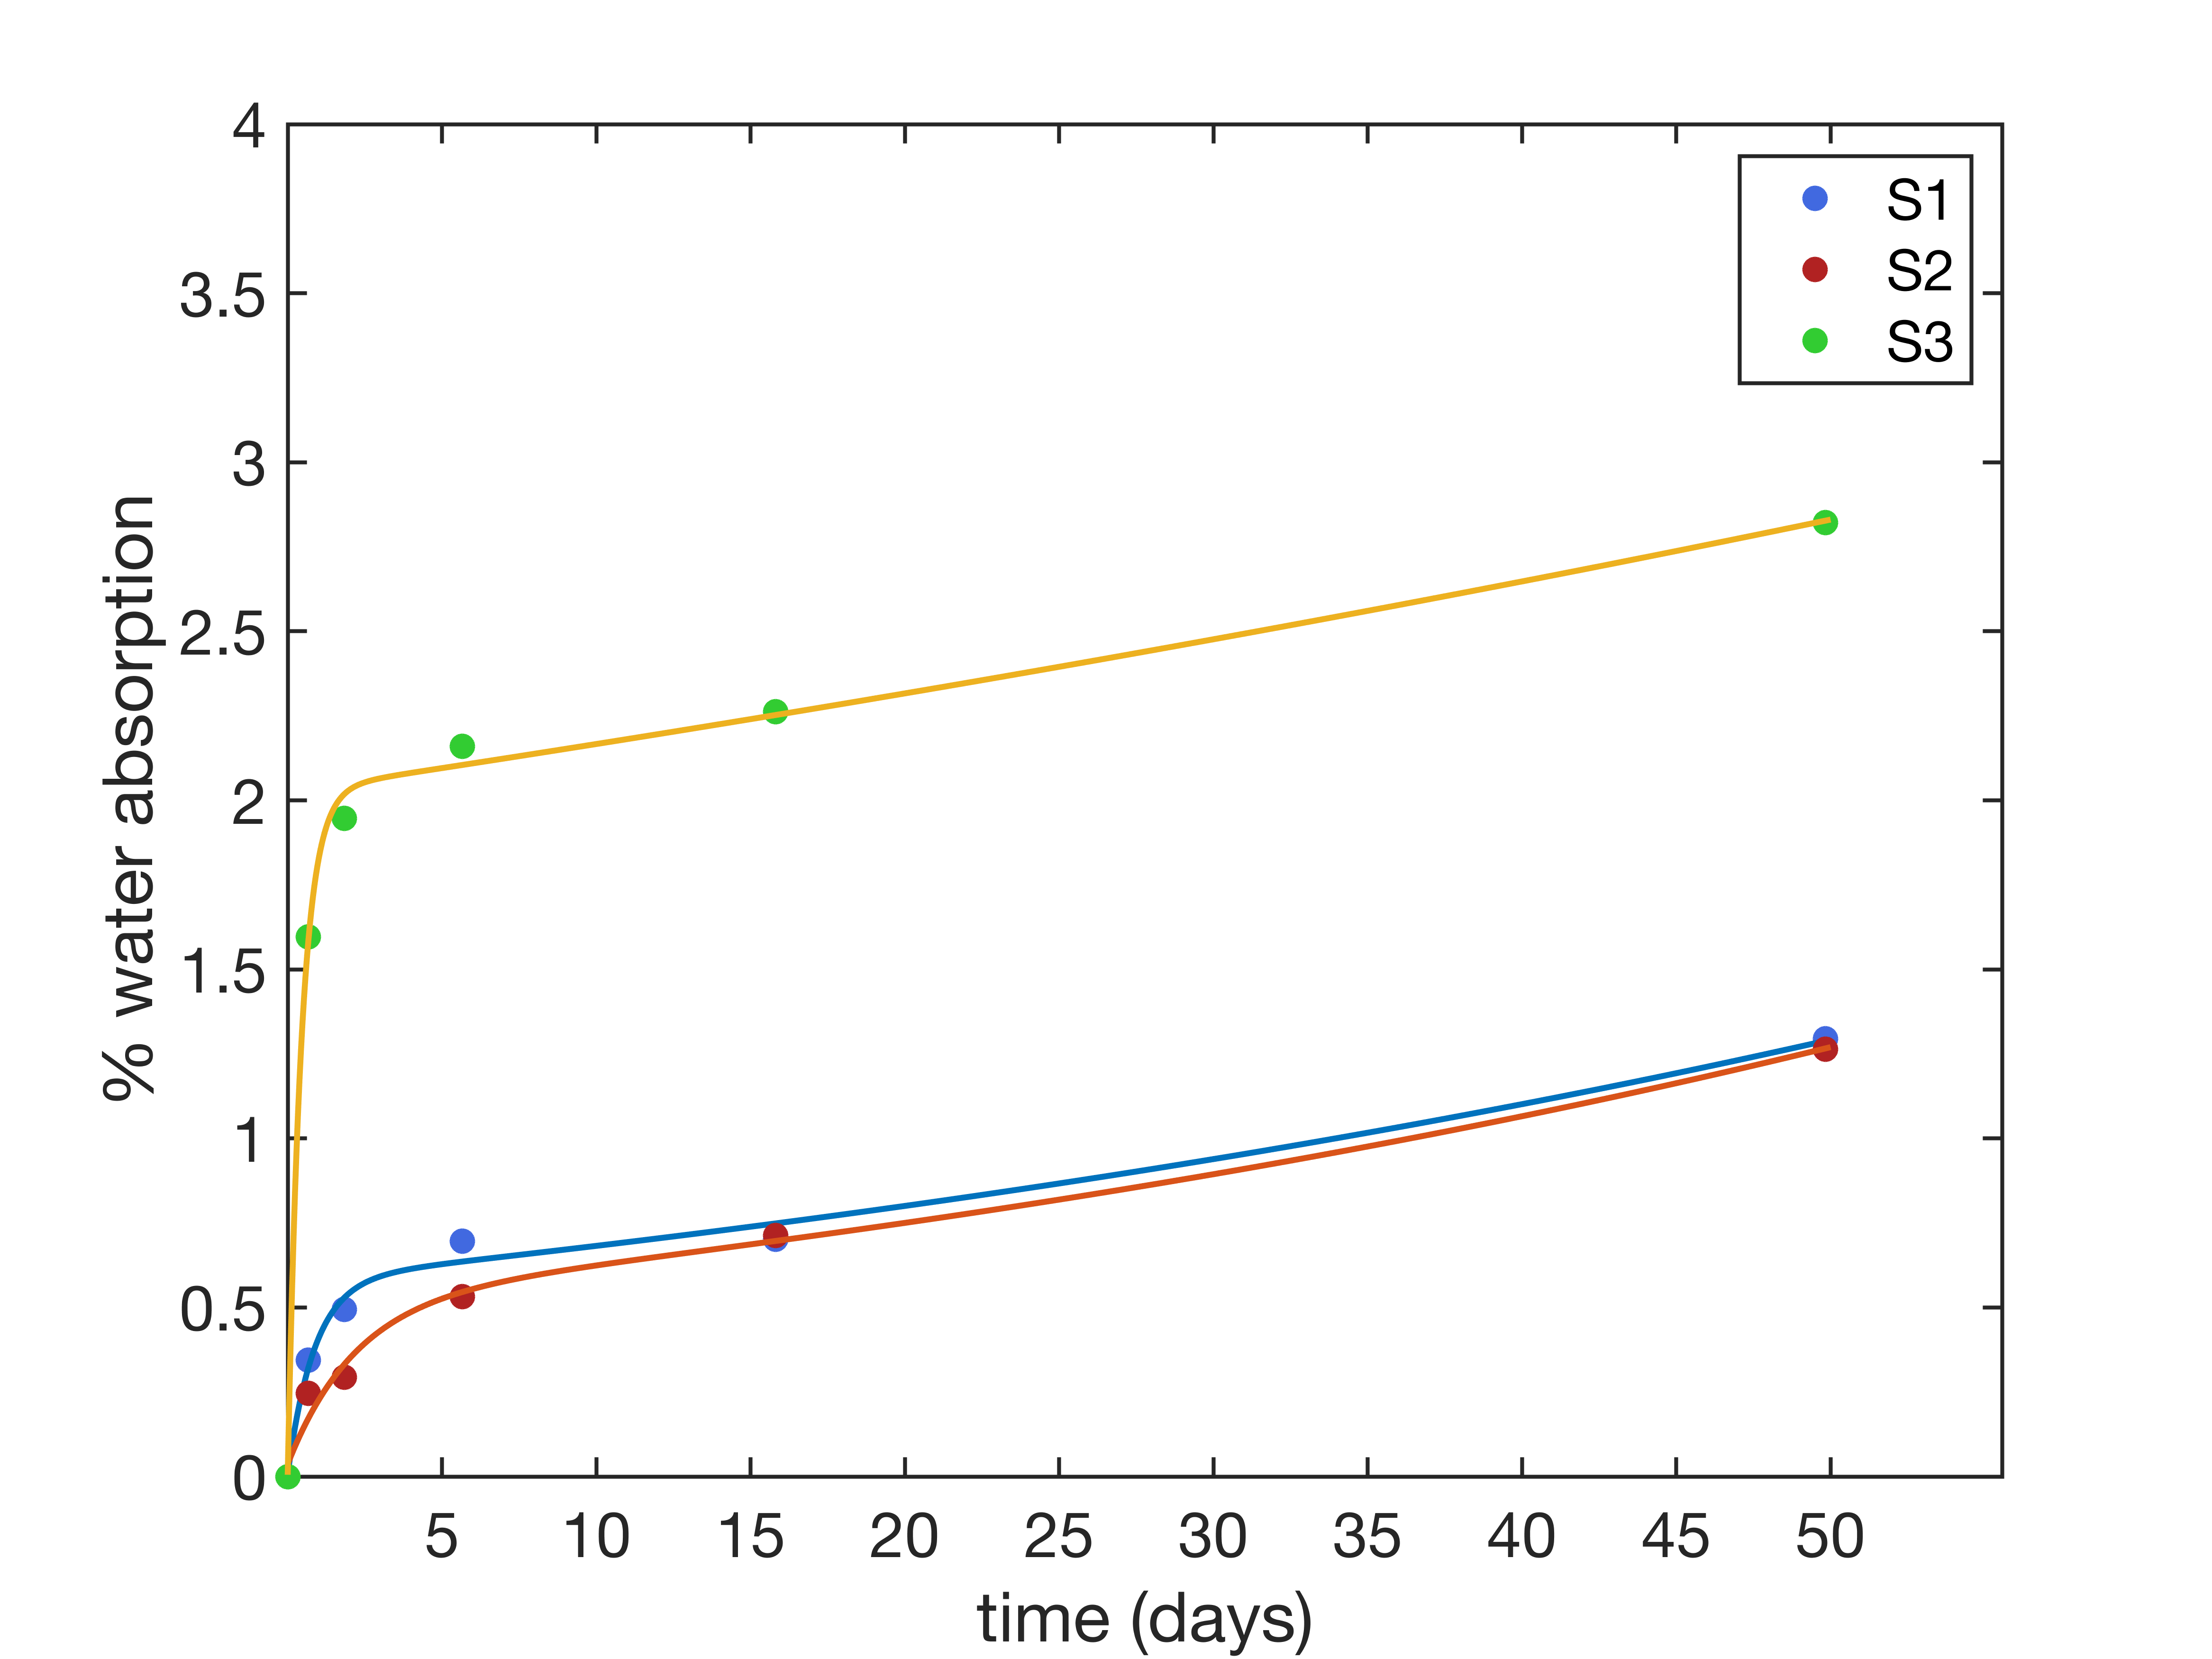
\includegraphics[scale=0.35]{wabs_s}}
\captionsetup{justification=centering}
\caption{Water absorption curves for samples S1, S2 and S3.}
\label{fig:wabs2}
\end{figure}

The second chart is the less precise. This can be explained by the poor control over the sample during processing, indeed polymerization has abruptly started still during formation, with strong release of heat (as seen also in heat of polymerization measurements, where the heat ramp starts from about $50^\circ$C) and thus poor control of the porosity. Manipulation and formation of the sample was stopped in favor of the temperature ramp measurement. The third sample S3 has a completely different behavior in water absorption with respect to S1 and S2. This can be related to a much higher amount of open porosity, macroscopically visible by sample examination. 
\newpage
Although this remarkable difference, literature results of PMMA water absorption are closer to S3 and sticks results, about 2\%. After about two weeks from initial soaking, the water absorption reaches a plateau. 

In Table \ref{tab:wabs} the results of water absorption for sticks and spheroids are reported, after 50 days from the soaking. 
\begin{table}[htp]
\centering
$
\begin{array}{lc}
\toprule
\textbf{Sample} & \textbf{$\%$water abs}  \\
\midrule
\text{P1} & 2.33 \pm0.18 \\
\text{P1HT} & 2.31\pm0.16 \\
\text{P2} & 3.05\pm0.09 \\
\text{P2HT} & 2.28\pm0.17 \\
\midrule
\text{S1} & 1.29 \\
\text{S2} & 1.26 \\
\text{S3} & 2.82 \\
\bottomrule
\end{array}
$
\caption{Water absorption measurements after 50 days from the soaking.}
\label{tab:wabs}
\end{table}\\

\subsubsection{Drying of samples after water soaking}

Dried samples percent weight losses are reported in Table \ref{tab:dried}. 
\begin{table}[htp]
\centering
$
\begin{array}{lc}
\toprule
\textbf{Sample} & \textbf{$\%$weight loss}  \\
\midrule
\text{P1} & -0.82 \pm0.02 \\
\text{P1HT} & -0.35\pm0.01 \\
\text{P2} & -0.67\pm0.24 \\
\text{P2HT} & -1.22\pm1.31 \\
\midrule
\text{S1} & -0.09 \\
\text{S2} & 0.02 \\
\text{S3} & -0.37 \\
\bottomrule
\end{array}
$
\caption{Weight losses after drying.}
\label{tab:dried}
\end{table}\\
The mass loss is related to the loss of unreacted monomer still present in the bone cement after three months. Of course a certain percent of it is present due to the always lower kinetics of polymerization in time, resulting in a certain degree of unreacted monomer even after very long times. The water soaking had the effect of taking place of the monomer inside the sample and diluting it in the solvent. During the drying process, water has evaporated, resulting in a net mass loss of the samples, compared to the initial one just after polymerization. 
The mass loss in heat treated sample not containing HEMA (P1HT) is significantly less than the others, a sign that the heat treatment have accelerated the polymerization reaction and the residual unreacted monomer is less. Instead, the heat treated sample containing HEMA is not very representative due to the too high standard deviation. Presence of HEMA in P2 sample is less than the P1 not containing HEMA. 

\section{Conclusions}

This laboratory activity has permitted to study the radical polymerization process, in order to achieve a better understanding of the theoretical concepts at the base of it.
In the second polymerization the heat released during the reaction is higher than the two other cases due to the presence of a larger amount of monomer MMA. It has also been noticed that the presence of HEMA doesn't influence the heat production. Moreover, the value of heat calculated in the first polymerization is comparable with the theoretical one. The third polymerization highlights that, due to the high surface/volume ratio, the heat dissipation is more significant. About molecular weight, as expected, in the first and third case the resulting values are almost equal, while in the second one are higher and this can be explained by the additional quantity of MMA to the base kit in the second polymerization process. The addition of HEMA at the beginning has led to an higher water absorption due to its hydrophilicity. From the heat treatment analysis it has been noticed a very slightly decrease of water absorption. This is due to the partial evaporation of non-polymerized monomer and to the higher degree of polymerization induced by the higher temperature.

\newpage

\begin{appendices}

\section{Heat treatement weight measurements}

\begin{table}[htp]
	\centering
	$
	\begin{array}{ccc}
	\toprule
	\textbf{Sample} & \bm{m_{i}} & \bm{m_{f}}\\
	\midrule
	\text{P1–B} & 2.6534 & 2.6498 \\
	\text{P1–C} & 2.1869 & 2.1841 \\
	\text{P2–B} & 3.0995 & 3.0969 \\
	\text{P2–C} & 2.3333 & 2.3304 \\
	\bottomrule
	\end{array}
	$
	\caption{Weight measurements before and after heat treatment.}
	\label{tab:weight}
\end{table}
Where ${m_{i}}$ is the mass of samples before heat treatment and ${m_{f}}$ is the mass of samples after heat treatment.

\end{appendices}

\newpage

\thispagestyle{empty}

\begin{thebibliography}{11}

\bibitem{link0} Sudipta Roy, Indian Institute of Technology-Bombay, Mumbai-400076, India. Calculation of heat of polymerisation: group-contribution method. Polymer Bulletin 42, 229–236 (1999).

\end{thebibliography}

\end{document}